\chapter{Agenda y Alertas}\label{cap:agenda-alertas}

% ---------------------------------------------------------------------
\section{Agenda}\label{sec:agenda}

\paraque Reúne en un calendario las audiencias y los vencimientos de plazos
de todos los expedientes a los que usted tiene acceso.

\disponible Administrador, Litigante y Asistente legal.

\pasos
\begin{enumerate}
  \item En el menú, haga clic en \textbf{Agenda}. Se abre la
        \textbf{Agenda del despacho} en la vista \textbf{Semana}.
  \item En \textbf{Vista de agenda}, elija \textbf{Día}, \textbf{Semana},
        \textbf{Mes} o \textbf{Rango personalizado}.
  \item Elija la \textbf{Fecha de referencia} (con su \textbf{Desfase de
        consulta}), o haga clic en un día del
        calendario que aparece junto a la lista; las flechas del calendario
        cambian el mes mostrado.
  \item En \textbf{Estado de audiencia} elija \textbf{Programadas},
        \textbf{Canceladas} o \textbf{Todas}. En \textbf{Tipo de actividad},
        elija qué mostrar:
        \textbf{Audiencias y plazos}, \textbf{Audiencias}, \textbf{Plazos},
        \textbf{Audiencias de recursos} o \textbf{Audiencias cautelares}.
  \item Haga clic en \textbf{Consultar Agenda}.
  \item Haga clic en una actividad de \textbf{Actividades en el periodo}
        para abrirla en su expediente.
\end{enumerate}

\begin{figure}[H]
  \centering
  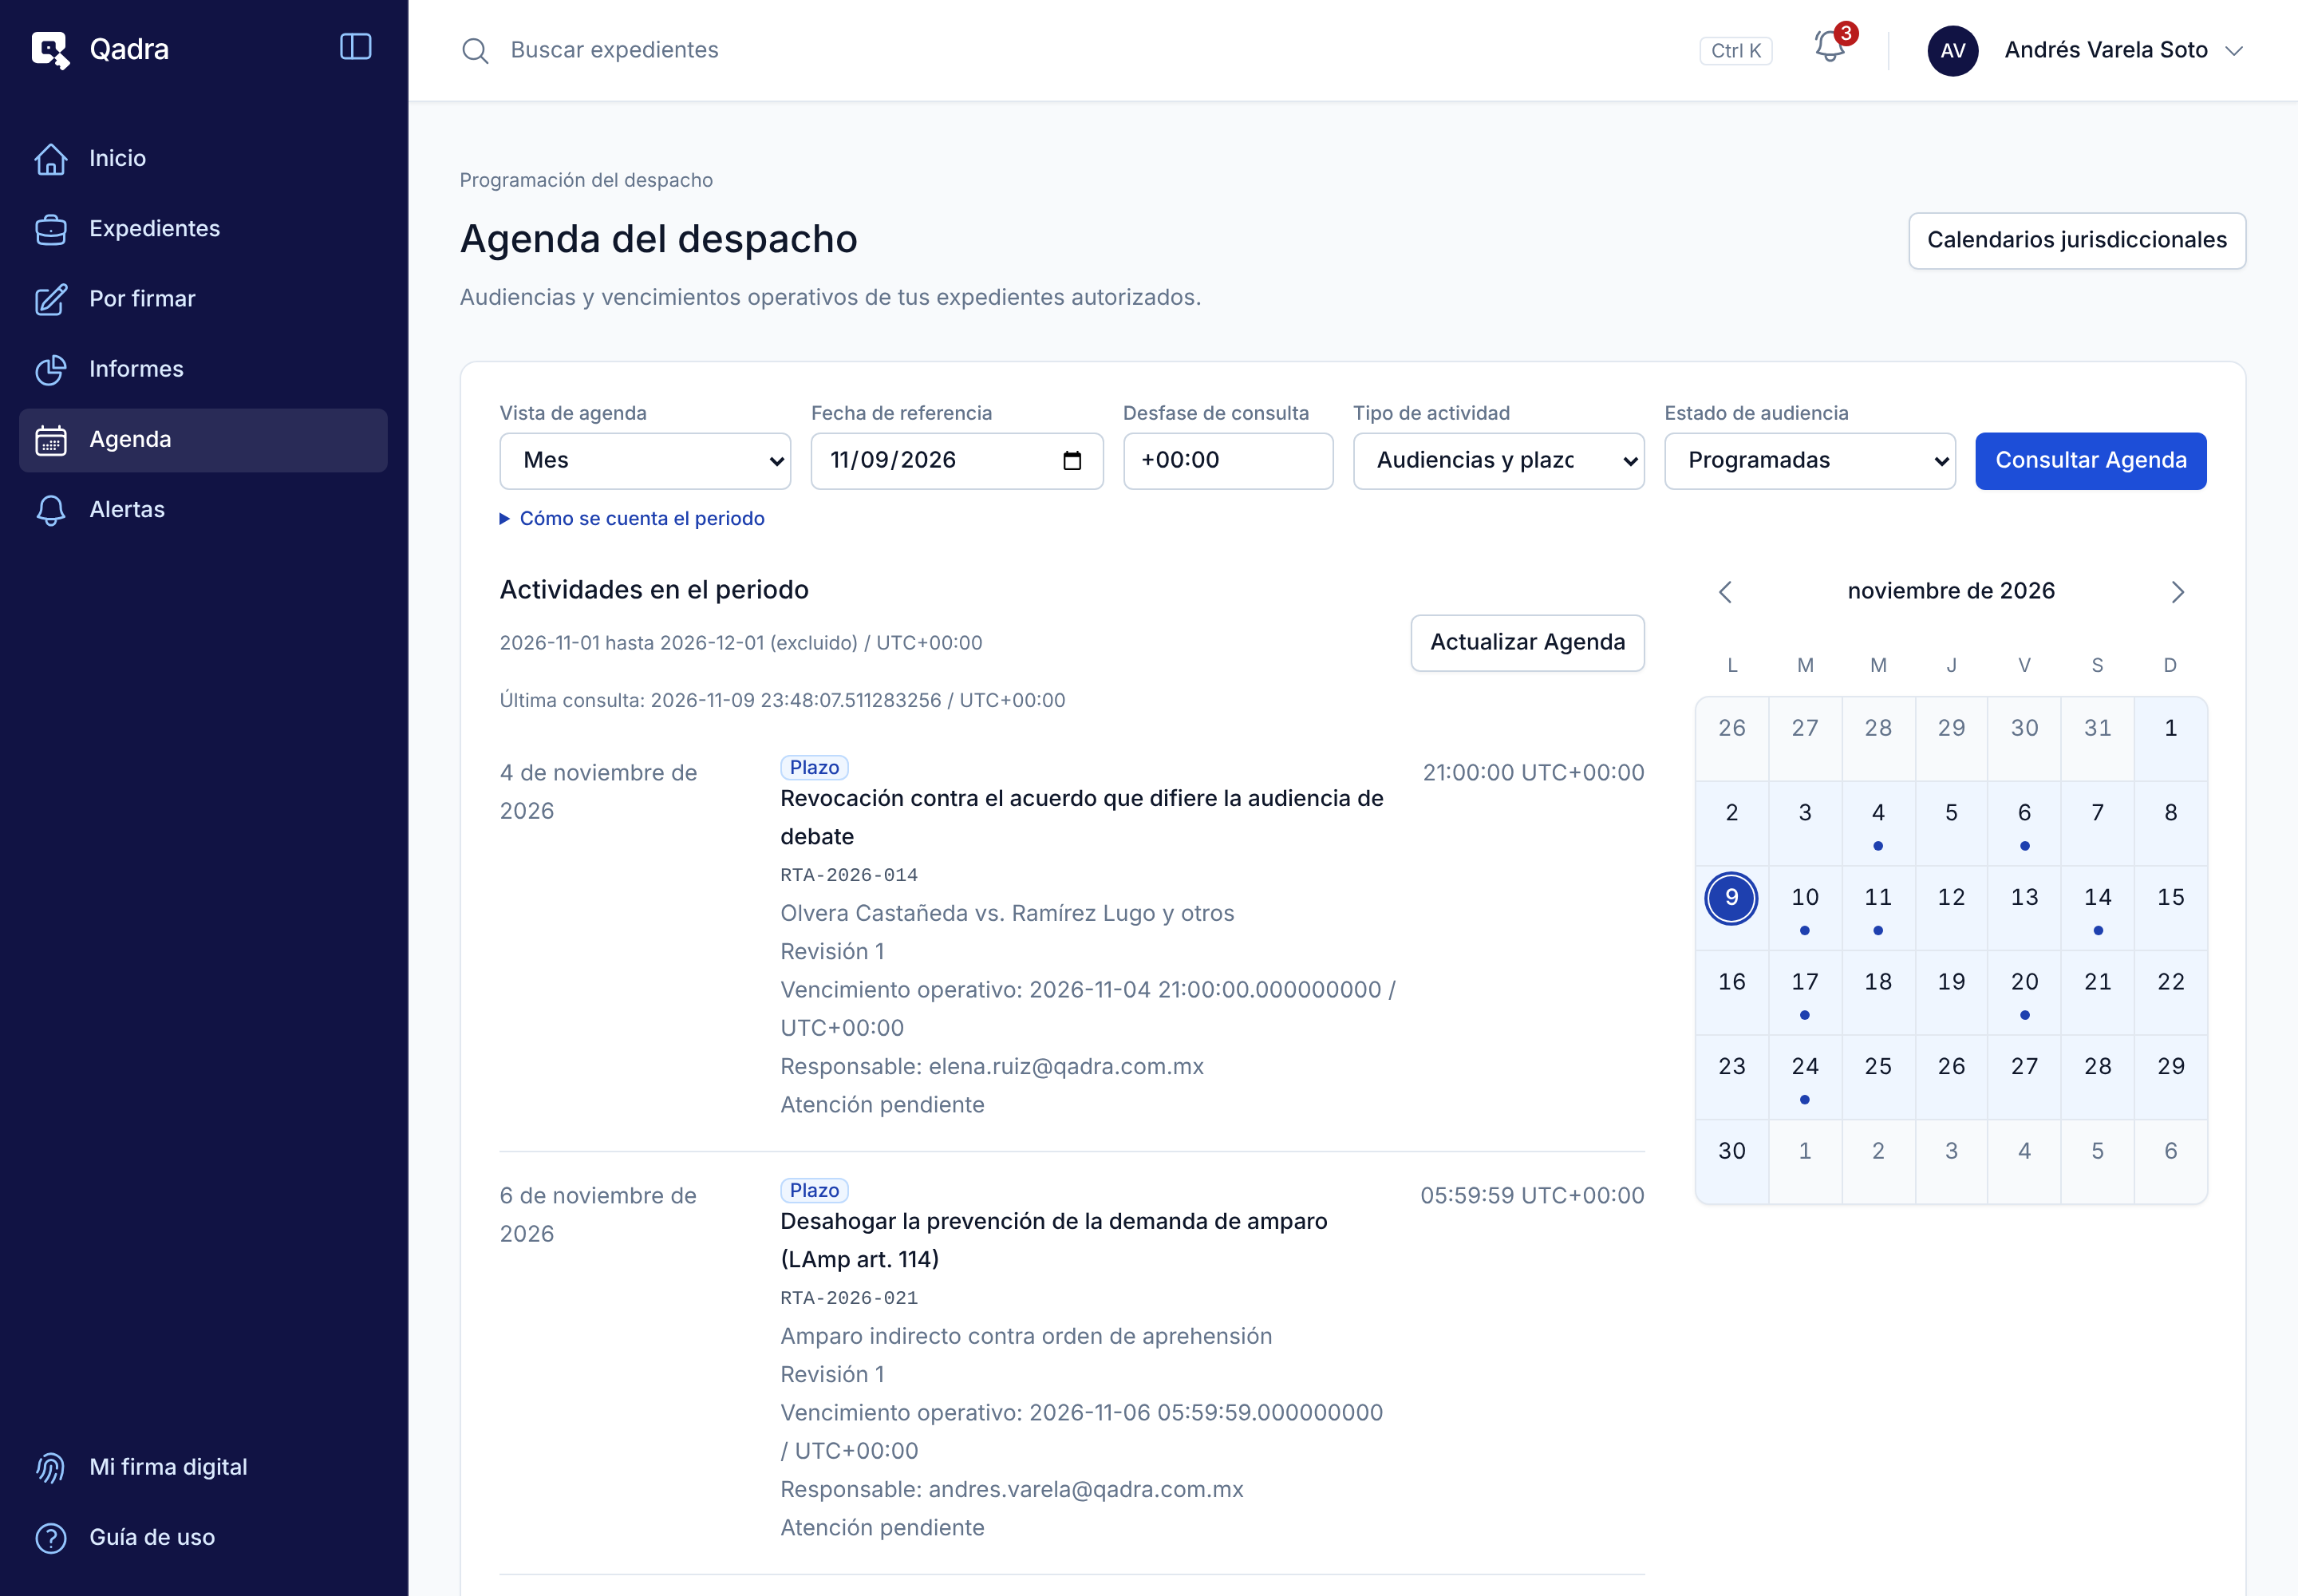
\includegraphics[width=0.9\textwidth,height=0.8\textheight,keepaspectratio]{capturas/A-34-agenda.png}
  \caption{Agenda del despacho.}
  \label{fig:manual-agenda}
\end{figure}

\resultado Ve sus audiencias y vencimientos del periodo, y abre cada uno en
un clic.

\begin{itemize}
  \item Si aparece \enquote{Consulta parcial: faltan actividades por
        consultar.}, haga clic en \textbf{Cargar más actividades}.
  \item Las actividades pueden cambiar entre consultas. Haga clic en
        \textbf{Actualizar Agenda} antes de tomar una decisión.
  \item Los plazos que requieren revisión no aparecen en la Agenda;
        consúltelos en la pestaña \textbf{Plazos} del expediente.
  \item El botón \textbf{Calendarios jurisdiccionales} muestra los días
        hábiles e inhábiles que usa Qadra para calcular plazos.
\end{itemize}

% ---------------------------------------------------------------------
\section{Alertas}\label{sec:alertas}

\paraque Muestra sus avisos personales sobre audiencias y plazos próximos,
vencidos o modificados.

\disponible Administrador, Litigante y Asistente legal. Cada persona ve solo
sus propias alertas.

\pasos
\begin{enumerate}
  \item En el menú, haga clic en \textbf{Alertas}, o en la campana de la
        barra superior. Se abre \textbf{Mis alertas}.
  \item Para ver solo lo pendiente, elija \textbf{Sin leer} en
        \textbf{Lectura} y haga clic en \textbf{Consultar alertas}.
  \item Haga clic en el botón de la alerta (\textbf{Abrir audiencia},
        \textbf{Abrir plazo}, etc.) para revisar su origen.
  \item Cuando la haya revisado, haga clic en \textbf{Marcar como leída}.
\end{enumerate}

\begin{figure}[H]
  \centering
  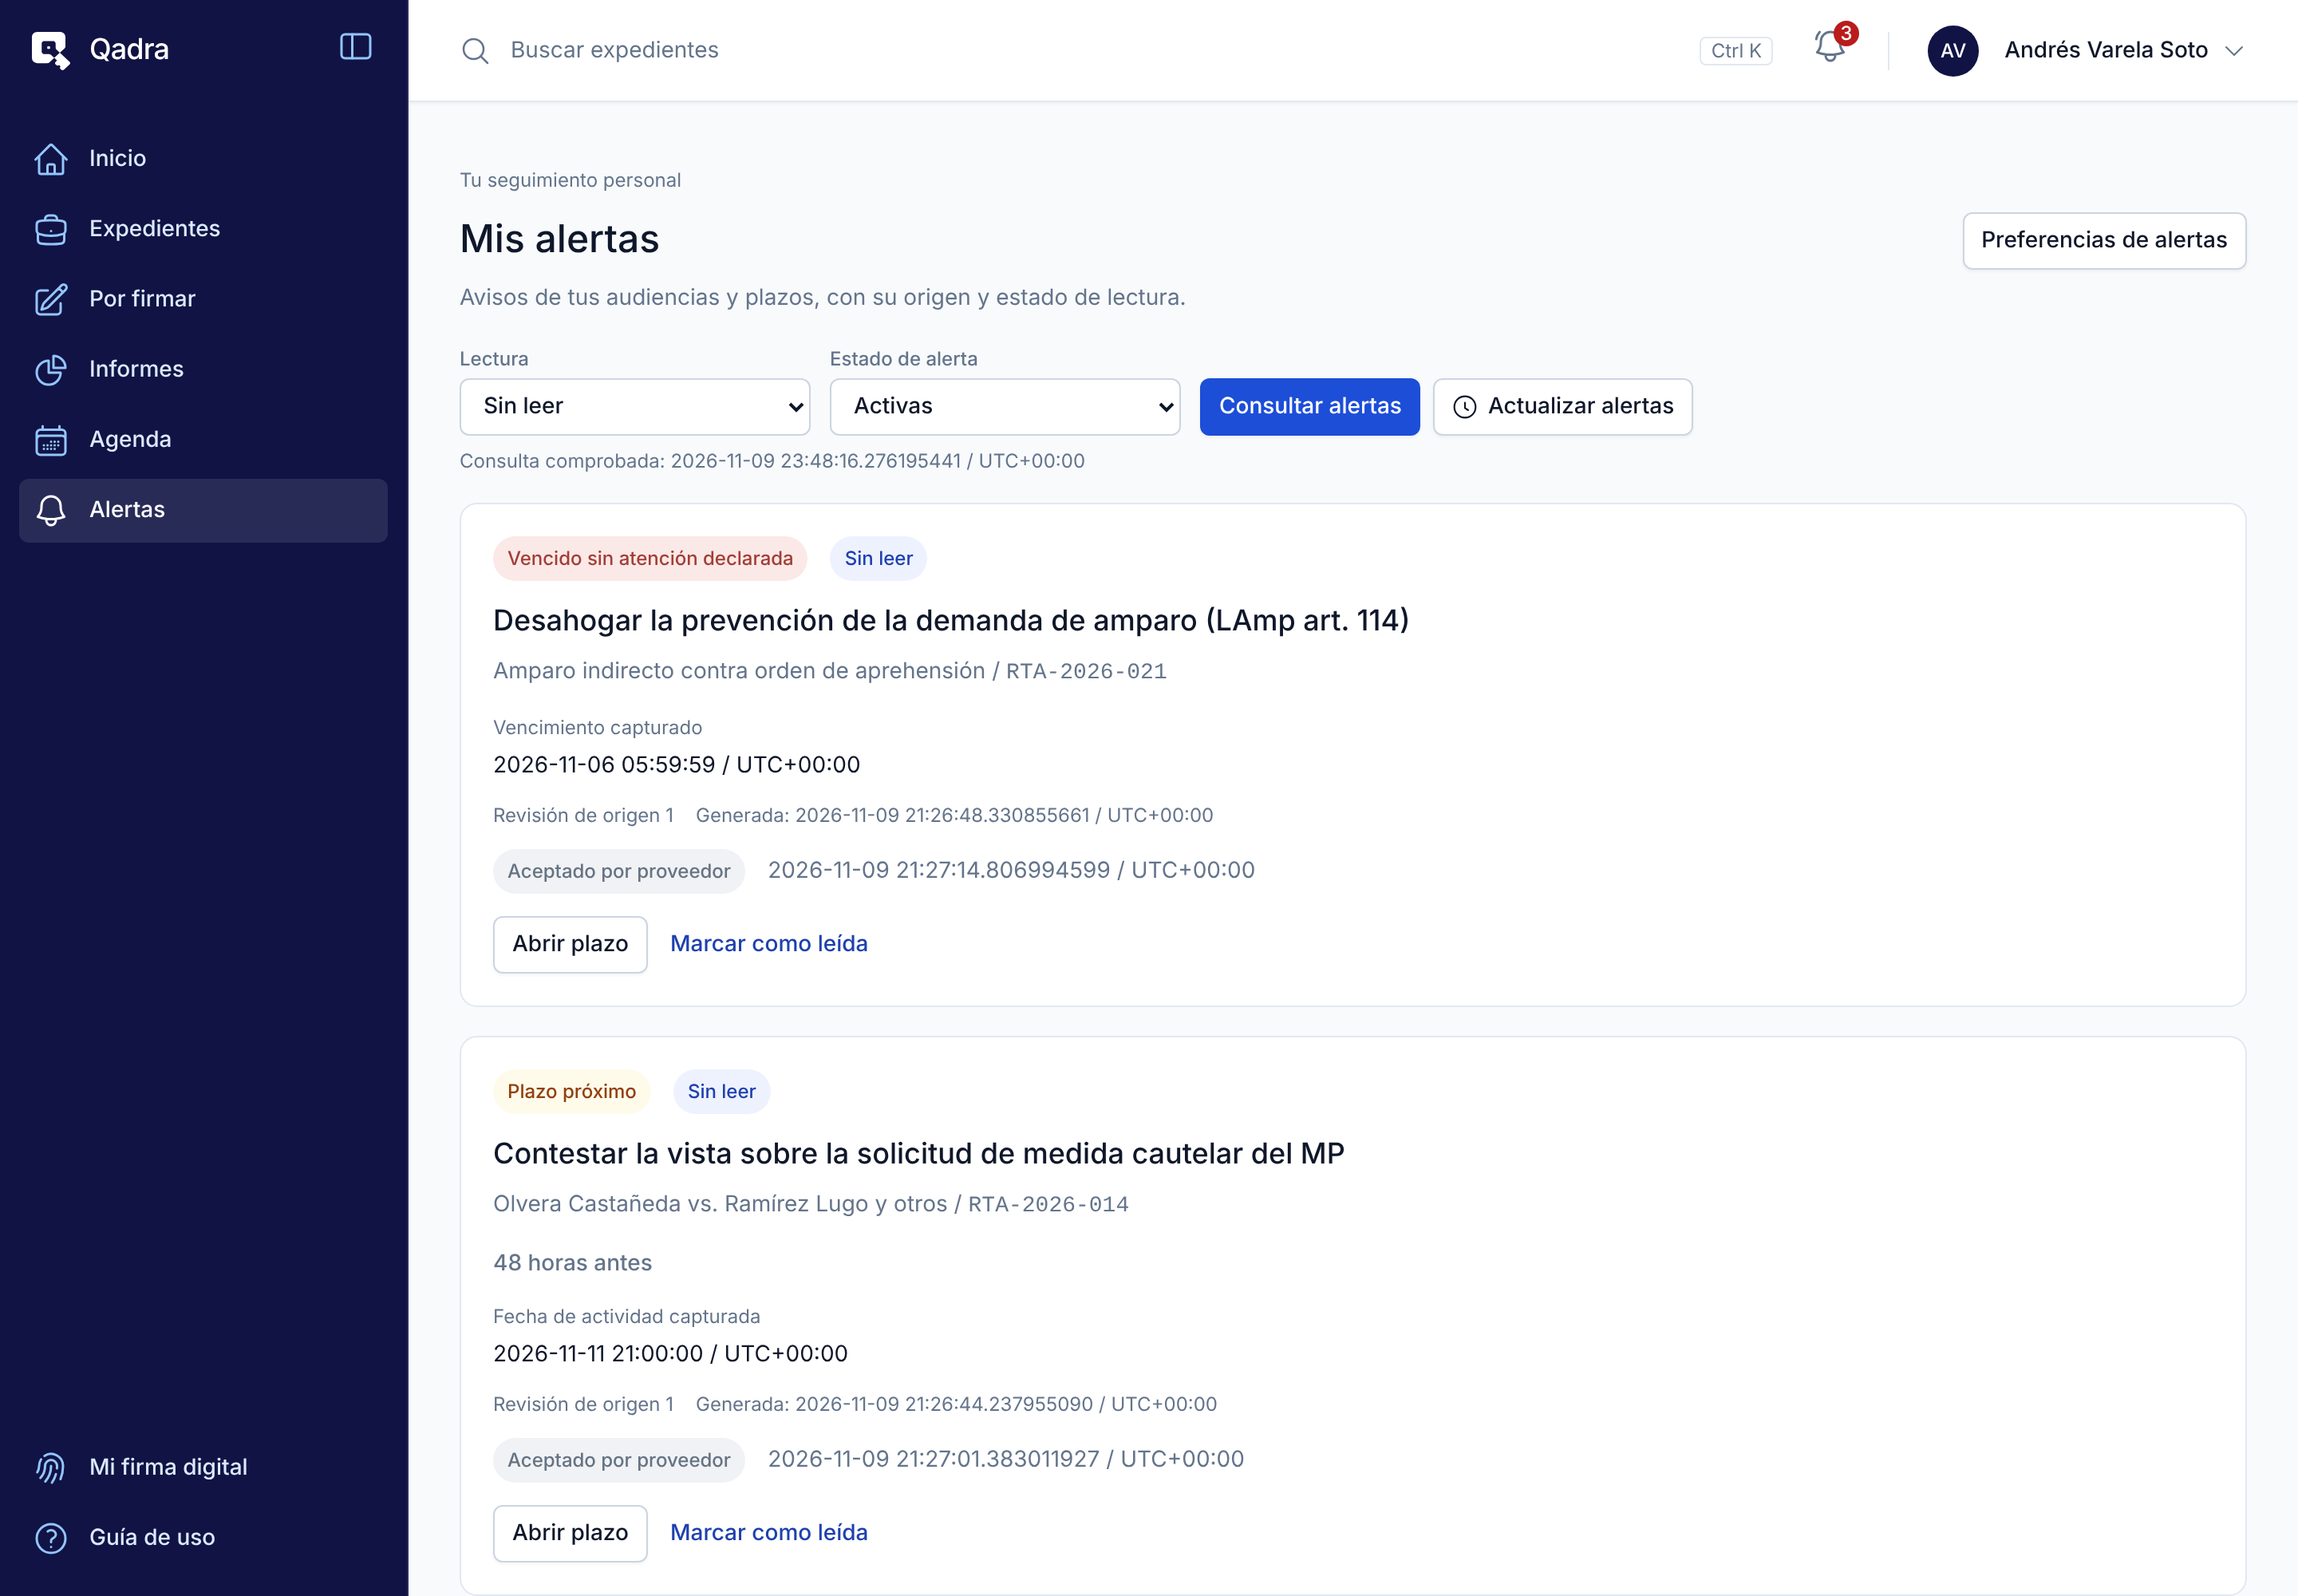
\includegraphics[width=0.9\textwidth,height=0.8\textheight,keepaspectratio]{capturas/A-35-mis-alertas.png}
  \caption{Bandeja de alertas.}
  \label{fig:manual-alertas}
\end{figure}

\resultado La alerta queda como \textbf{Leída}.

\begin{table}[H]
  \centering
  \caption{Tipos de alerta.}\label{tab:tipos-alerta}
  \begin{tabularx}{\textwidth}{L{5.2cm} Y}
    \toprule
    \textbf{Alerta} & \textbf{Cuándo aparece} \\
    \midrule
    \textbf{Audiencia próxima} (también cautelar o de recurso) & Se acerca una audiencia. \\
    \textbf{Plazo próximo}                     & Se acerca un vencimiento. \\
    \textbf{Vencido sin atención declarada}    & Venció un plazo y nadie declaró su atención. \\
    \textbf{Revisión requerida}                & Un plazo necesita que lo revise. \\
    \textbf{Fecha próxima modificada}          & Cambió la fecha de una actividad cercana. \\
    \bottomrule
  \end{tabularx}
\end{table}

\nota{Abrir una alerta no la marca como leída; use el botón
\textbf{Marcar como leída}. Leer una alerta tampoco declara la atención del
plazo.}

\subsection*{Preferencias de alertas}

\pasos
\begin{enumerate}
  \item En \textbf{Mis alertas}, vaya a \textbf{Preferencias de alertas}.
  \item Para cada grupo (\textbf{Audiencias próximas},
        \textbf{Plazos próximos}, etc.), marque si quiere avisos internos y
        por correo.
  \item En las anticipaciones, escriba con cuántas horas de anticipación
        quiere el aviso: hasta ocho valores entre 1 y 720, separados por
        comas (por ejemplo, \texttt{24, 72}).
  \item Haga clic en \textbf{Guardar preferencias}.
\end{enumerate}

\resultado Aparece \enquote{Preferencias guardadas.}

\nota{El correo solo contiene un aviso genérico y el acceso a Qadra, sin
datos del expediente. Si el servidor no tiene el correo habilitado, sus
preferencias se guardan pero no se envían correos.}
